\documentclass{article}
\usepackage{float}
\usepackage{tikz}
\usepackage{colortbl}
\usetikzlibrary{decorations.pathreplacing}
\usetikzlibrary{positioning}
\usetikzlibrary{shapes}
\title{BSDCONV}
\date{}
\begin{document}
	\maketitle
	\tableofcontents
	\section{Syntax}
		\subsection{Phases \& Cascade}
			\begin{figure}[H]
				\centering
				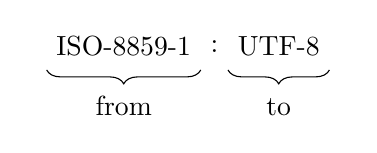
\begin{tikzpicture}[auto,node distance=0,on grid=false]

				    % Place nodes
				    \node (d0) {};
				    \node [right=of d0](from) {ISO-8859-1};
				    \node [right=of from](d1) {:};
				    \node [right=of d1] (to) {UTF-8};
				    \node [right=of to] (d2) {};
					
					\draw [decorate,decoration={brace,amplitude=5pt,raise=3mm, mirror}]
(d0)--(d1)  node  [black,midway,yshift=-1cm] { from };
				
					\draw [decorate,decoration={brace,amplitude=5pt,raise=3mm, mirror}]
(d1) -- (d2)  node [black,midway,yshift=-1cm] { to };
				
				\end{tikzpicture}
				\caption{Basic two phases conversion}
			\end{figure}
			
			\begin{figure}[H]
				\centering
				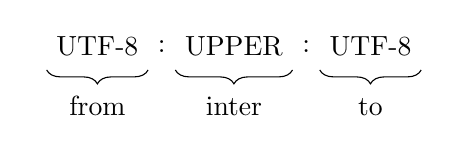
\begin{tikzpicture}[auto,node distance=0,on grid=false]			
				    % Place nodes
				    \node (d0) {};
				    \node [right=of d0](from) {UTF-8};
				    \node [right=of from](d1) {:};
				    \node [right=of d1] (inter) {UPPER};
				    \node [right=of inter](d2) {:};
				    \node [right=of d2] (to) {UTF-8};
				    \node [right=of to] (d3) {};			
					
					\draw [decorate,decoration={brace,amplitude=5pt,raise=3mm, mirror}]
	(d0) -- (d1) node [black,midway,yshift=-1cm] { from };
					
					\draw [decorate,decoration={brace,amplitude=5pt,raise=3mm, mirror}]
	(d1) -- (d2) node [black,midway,yshift=-1cm] { inter };
					
					\draw [decorate,decoration={brace,amplitude=5pt,raise=3mm, mirror}]
	(d2) -- (d3) node [black,midway,yshift=-1cm] { to };
				\end{tikzpicture}
				\caption{Conversion with inter-mapping phase}
			\end{figure}
			
			\begin{figure}[H]
				\centering
				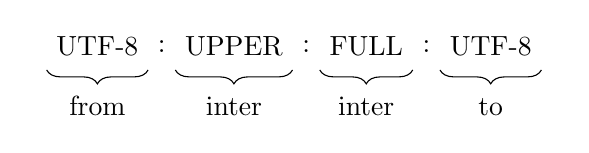
\begin{tikzpicture}[auto,node distance=0,on grid=false]
				    % Place nodes
				    \node (d0) {};
				    \node [right=of d0](from) {UTF-8};
				    \node [right=of from](d1) {:};
				    \node [right=of d1] (inter) {UPPER};
				    \node [right=of inter](d2) {:};
				    \node [right=of d2] (inter2) {FULL};
				    \node [right=of inter2](d3) {:};
				    \node [right=of d3] (to) {UTF-8};
				    \node [right=of to] (d4) {};			
					
					\draw [decorate,decoration={brace,amplitude=5pt,raise=3mm, mirror}]
	(d0) -- (d1) node [black,midway,yshift=-1cm] { from };
					
					\draw [decorate,decoration={brace,amplitude=5pt,raise=3mm, mirror}]
	(d1) -- (d2) node [black,midway,yshift=-1cm] { inter };
					
					\draw [decorate,decoration={brace,amplitude=5pt,raise=3mm, mirror}]
	(d2) -- (d3) node [black,midway,yshift=-1cm] { inter };
					
					\draw [decorate,decoration={brace,amplitude=5pt,raise=3mm, mirror}]
	(d3) -- (d4) node [black,midway,yshift=-1cm] { to };
				
				\end{tikzpicture}
				\caption{Conversion with multiple inter-mapping phases}
			\end{figure}
	
			\begin{figure}[H]
				\centering
				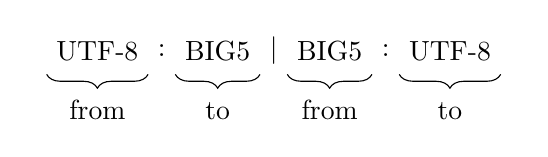
\begin{tikzpicture}[auto,node distance=0,on grid=false]
				    % Place nodes
				    \node (d0) {};
				    \node [right=of d0] (from) {UTF-8};
				    \node [right=of from] (d1) {:};
				    \node [right=of d1] (to) {BIG5};
				    \node [right=of to] (d2) {$|$};
				    \node [right=of d2] (from2) {BIG5};
				    \node [right=of from2](d3) {:};
				    \node [right=of d3](to2) {UTF-8};
				    \node [right=of to2] (d4) {};
					
					\draw [decorate,decoration={brace,amplitude=5pt,raise=3mm, mirror}] (d0) -- (d1) node [black,midway,yshift=-1cm] { from };
				
					\draw [decorate,decoration={brace,amplitude=5pt,raise=3mm, mirror}] (d1) -- (d2) node [black,midway,yshift=-1cm] { to };

					\draw [decorate,decoration={brace,amplitude=5pt,raise=3mm, mirror}] (d2) -- (d3) node [black,midway,yshift=-1cm] { from };

					\draw [decorate,decoration={brace,amplitude=5pt,raise=3mm, mirror}] (d3) -- (d4) node [black,midway,yshift=-1cm] { to };
				
				\end{tikzpicture}
				\caption{Cascaded conversions}
			\end{figure}
		
		\subsection{Codecs \& Fallback}
			\begin{figure}[H]
				\centering
				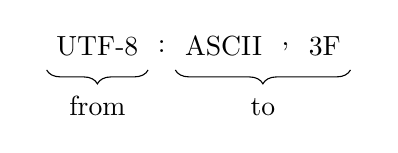
\begin{tikzpicture}[auto,node distance=0,on grid=false]
				    % Place nodes
				    \node (d0) {};
				    \node [right=of d0] (from) {UTF-8};
				    \node [right=of from] (d1) {:};
				    \node [right=of d1] (to) {ASCII};
				    \node [right=of to] (d2) {,};
				    \node [right=of d2] (from2) {3F};
				    \node [right=of from2] (d3) {};
					
					\draw [decorate,decoration={brace,amplitude=5pt,raise=3mm, mirror}] (d0) -- (d1) node [black,midway,yshift=-1cm] { from };
				
					\draw [decorate,decoration={brace,amplitude=5pt,raise=3mm, mirror}] (d1) -- (d3) node [black,midway,yshift=-1cm] { to };
				
				\end{tikzpicture}
				\caption{Fallback codec}
			\end{figure}
			
		\subsection{Codec argument}
			\begin{figure}[H]	
				\centering
				\begin{tikzpicture}[auto,node distance=0,on grid=false]
				    % Place nodes
				    \node (d0) {};
				    \node [right=of d0] (from) {UTF-8};
				    \node [right=of from] (d1) {:};
				    \node [right=of d1] (to) {ASCII};
				    \node [right=of to] (d2) {,};
				    \node [right=of d2] (to2) {ANY\#3F};
				    \node [right=of from2] (d3) {};
				
				\end{tikzpicture}
				\caption{Passing argument to codec}
			\end{figure}
			
			\begin{figure}[H]
				\centering
				
\begin{tikzpicture}[auto,node distance=0,on grid=false]
				    % Place nodes
				    \node (d0) {};
				    \node [right=of d0](from) {UTF-8};
				    \node [right=of from](d1) {:};
				    \node [right=of d1] (to) {ASCII};
				    \node [right=of to] (d2) {,};
				    \node [right=of d2] (to2) {ESCAPE\#PREFIX=2575};
				    \node [right=of to2] (d3) {};
				
				\end{tikzpicture}
				\caption{Passing argument to codec in key=value form}
			\end{figure}
			
			\begin{figure}[H]
				\centering
				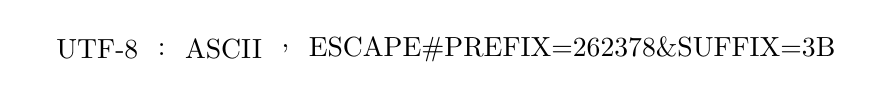
\begin{tikzpicture}[auto,node distance=0,on grid=false]
				    % Place nodes
				    \node (d0) {};
				    \node [right=of d0](from) {UTF-8};
				    \node [right=of from](d1) {:};
				    \node [right=of d1] (to) {ASCII};
				    \node [right=of to] (d2) {,};
				    \node [right=of d2] (to2) {ESCAPE\#PREFIX=262378\&SUFFIX=3B};
				    \node [right=of to2] (d3) {};
				
				\end{tikzpicture}
				\caption{Passing multiple arguments to codec}
			\end{figure}
	\clearpage
	\section{Type \& Flag}
		\subsection{Type}
			\paragraph{}
				\begin{table}[H]
					\centering
					\begin{tabular}{|>{\columncolor{blue!30}}c | l | c | c|}
						\hline
						ID & Description & Provider(from) & Consumer(to)\\
						\hline
						00 & Bsdconv special characters & BSDCONV\_KEYWORD & BSDCONV\_KEYWORD\\
						01 & Unicode & Most decoder & Most encoder\\
						02 & CNS11643\footnotemark[1] & CNS11643 & CNS11643\\
						03 & Byte & BYTE; ESCAPE & BYTE; ESCAPE\#MODE=\{8,16\}\\
						04 & Chinese components & inter/ZH\_DECOMP & inter/ZH\_COMP\\
						1B & ANSI control sequence & ANSI-CONTROL & -\\
						\hline
					\end{tabular}
					\caption{Types and its provider/consumer (just to name a few)}
				\end{table}
				\footnotetext[1]{As for the intersection of CNS11643 and Unicode, from/CNS11643 does conversion to unicode type if possible. Vice versa, to/CNS11643 does conversion from unicode type if possible.}
				\begin{figure}[H]
					\centering
					\begin{tikzpicture}[auto,node distance=1.5cm,on grid=false]
					    % Place nodes
					    \node [rectangle,draw] (input) {A$\forall$};
					    \node [below=0 of input] {Input (UTF-8 literal)};
					    \node [ellipse,draw,right=of input] (decoder) {ASCII,BYTE : ...};
					    \node [below=0 of decoder] {Decoder};
						\tikzstyle{data} = [rectangle, draw,    text width=2em, text centered]
					    \node [rectangle,draw,right=of decoder] (internal) {
							\begin{tikzpicture}[node distance=3mm]
								\node [data,fill=blue!30](n0){01};
								\node [below=0 of n0,data](n1){41};
								\node [right=of n0,data,fill=blue!30](n2){03};
								\node [below=0 of n2,data](n3){E2};
								\node [right=of n2,data,fill=blue!30](n4){03};
								\node [below=0 of n4,data](n5){88};
								\node [right=of n4,data,fill=blue!30](n6){03};
								\node [below=0 of n6,data](n7){80};
								\draw [->] (n0) -- (n2);
								\draw [->] (n2) -- (n4);
								\draw [->] (n4) -- (n6);
							\end{tikzpicture}
					    };
					    \node [below=0 of internal] {Internal data};
					    \node [ellipse,draw,below=3cm of input] (encoder) {... : ASCII,ESCAPE};
					    \node [below=0 of encoder] {Encoder};
					    					    \node [rectangle,draw,right=of encoder] (internal2) {
							\begin{tikzpicture}[node distance=3mm]
								\node [data](n0){41};
								\node [above=0 of n0]{"A"};
								\node [right=of n0,data](n1){25};
								\node [below=0 of n1,data](n2){45};
								\node [below=0 of n2,data](n3){32};
								\node [above=0 of n1]{"\%E2"};
								\node [right=of n1,data](n4){25};
								\node [below=0 of n4,data](n5){38};
								\node [below=0 of n5,data](n6){38};
								\node [above=0 of n4]{"\%88"};
								\node [right=of n4,data](n7){25};
								\node [below=0 of n7,data](n8){38};
								\node [below=0 of n8,data](n9){30};
								\node [above=0 of n7]{"\%80"};
								\draw [->] (n0) -- (n1);
								\draw [->] (n1) -- (n4);
								\draw [->] (n4) -- (n7);
							\end{tikzpicture}
					    };
					    \node [below=0 of internal2] {Internal data};
					    \node [rectangle,draw,right=of internal2] (output) {A\%E2\%88\%80};
					    \node [below=0 of output] {Output (UTF-8 literal)};
					
						\draw [->] (input) -- (decoder);
						\draw [->] (decoder) -- (internal);
						\draw [->] (internal.east) -- ++ (0.5,0) -- ++ (0,-2) -| (encoder.north);
						\draw [->] (encoder) -- (internal2);
						\draw [->] (internal2) -- (output);
					\end{tikzpicture}
					\caption{Fallback \& Type}
				\end{figure}
		\subsection{Flag}
\end{document}
